In this section we introduce the usage of AFES by the use of examples. The AFES
api is written solely in Python (with the exception of UFL for the weak form)
and thus the user is expected to have a basic knowledge of Python programming.
However, since AFES is based on the FEniCS/DOLFIN Python interface it does not
compromise on performance\cite{Alnae2011}. The use of DOLFIN's Python interface
allows for greater ease of use, as compared to the C++ interface. Eventually, we
intend to offer a GUI which would require the use of no programming and only
entering the details for the domain, boundary conditions, and the weak form.

\subsection{Solving a PDE} \label{sse:Solver}

    In this subsection we explain how to solve a basic time dependent PDE using
    the AFES API. We choose to explain the API by example; we choose to
    make things quite simple at first and so the first example is the Heat
    equation.  Since, the FEM requires the weak form of any PDE we assume
    the user understands how to determine the weak form for a given PDE and thus
    no explanation of the weak form is given. For a very basic explanation of
    the weak form see \cite[Chapter 6.2.2]{Eriksson2009}.

    Of course to be able to solve any PDE certain assumptions must be made. AFES
    makes the assumption that an $H^1$ FE is appropriate for solving the given
    PDE, i.e. the FE discretization is stable. Additionally, AFES assumes the
    PDE has the following form
    \begin{equation}
        R(u) = u_t - F(u;t) = 0,
        \label{eq:BasicForm}
    \end{equation}
    and can be discretized in time in the following way
    \begin{equation}
        r(u^n, u^n, v) = \frac{1}{k} (u^n - u^{n-1}, v) - (F(\hat{u};t^n), v) = 0,
        \label{eq:WeakResidual}
    \end{equation}
    where $u^n,\, u^{n-1},\, \hat{u}$, and $v$ are the solution at the
    $n^{th}$-timestep, the solution at the $(n-1)^{st}$-timestep,
    $\theta$-weighted average of the solution for the $n^{th}$ and
    $(n-1)^{th}$-timestep, i.e.
    \begin{equation}
        \hat{u} = \theta\, u^n + (1 - \theta)\, u^{n-1},
        \label{eq:uAvg}
    \end{equation}
    and the test function, respectively.

    For AFES, a PDE is defined using the following required objects\slash
    functions \texttt{Problem.T}, \texttt{Problem.t0}, \texttt{Problem.k},
    \texttt{Problem.mesh}, \texttt{Problem.initial\_condition},
    \texttt{Problem.boundary\_conditions}, \texttt{Solver.function\_space}, and
    \texttt{Solver.weak\_residual}, which are the final time (float), initial
    time (float), time-step (float), domain discretization (mesh object),
    initial condition (function), boundary conditions (function), finite element
    space (function), and weak form (function), respectively. The function
    \texttt{Problem.initial\_condition} should return a finite element
    projection of the initial condition, while
    \texttt{Problem.boundary\_conditions} return a list of FEniCS
    \texttt{DirichletBC} objects. Then the function
    \texttt{Solver.function\_space} returns either a \texttt{FunctionSpace}
    object or a \texttt{MixedFunctionSpace} object. The user need not worry too
    much about the definition these FEniCS objects, but one must know to return
    these types when writing their functions. These details will become much
    clearer in the following subsections, where we will focus on the definition
    of these objects\slash functions and their use.

\subsubsection{Heat Equation} \label{sss:Heat}
    The heat equation is a canonical example of parabolic partial differential
    equations. Given the domain $\Omega$ with boundary $\partial \Omega$ and
    time interval $I$ the heat equation is given by
    \begin{equation}
        \begin{split}
            u_t - \nabla \left( \kappa \nabla u \right) &= f
                \qquad (\mathbf{x}, t)\in \Omega \times I \\
            u(\mathbf{x}, 0) &= u_0(\mathbf{x}) \quad \mathbf{x} \in \Omega \\
            u(\mathbf{x}, t) &= g(\mathbf{x},t) \quad (\mathbf{x}, t)\in
                \partial\Omega \times I, \\
        \end{split}
        \label{eq:Heat}
    \end{equation}
    where $f$ is the internal heat source/sink and $g$ is the boundary
    condition. Taking our FE basis functions $v_h\in V^h\subset H^1_0(\Omega)$
    then we are trying to find a $u^n_h \in V^h \subset H^1(\Omega)$ such that
    \begin{equation}
        \frac{1}{k} (u^n - u^{n-1}, v_h) + (\kappa \nabla \hat{u}, \nabla v_h) =
        0 \quad \forall v_h \in V^h,
        \label{eq:WeakHeat}
    \end{equation}
    where $k$ is the time step, $u^n_h$ is the FE solution at the
    $n^{th}$-timestep, $u^{n-1}_h$ is the FE solution at the
    $(n-1)^{st}$-timestep, $\hat{u}$ is given by \eqref{eq:uAvg}, and $\kappa$
    is the heat coefficient. To further
    specify the problem we will define the domain to be the unit square, i.e.
    \begin{equation}
        \Omega := [0, 1] \times [0, 1],
        \label{eq:HeatDomain}
    \end{equation}
    let the initial condition be
    \begin{equation}
        u0 := \sin(pi\, x)\, \sin(pi\, y)
        \label{eq:HeatIC}
    \end{equation}
    define the function to be
    \begin{equation}
        f(x,y,t) := 0
        \label{eq:HeatSource}
    \end{equation}
    and the boundary condition to be
    \begin{equation}
        g(x,y,t) := 0
        \label{eq:HeatBC}
    \end{equation}

    Just as in the definition of the PDE AFES requires certain things to be
    defined. First, we can define the mesh (we will use a
    \texttt{UnitSquareMesh} as our domain), and then the mesh must be passed to
    the \texttt{Problem} class. This can be done in the following way
    \lstinputlisting[firstline=63,lastline=68,
        caption={Creating a mesh of unit square problem domain.}
    ]{Heat.py}
    we need to define the initial conditions and
    boundary conditions. For the initial condition, \eqref{eq:HeatIC}, and
    the boundary condition, \eqref{eq:HeatBC}, these functions can be defined
    as follows
    \lstinputlisting[firstline=10,lastline=20,
        caption={Create the initial conditions and boundary conditions.}
    ]{Heat.py}
    To be able to access these functions AFES needs them define. To do this we
    must pass the functions to AFES' \texttt{Problem} class. This is done quite
    easily in the following way
    \lstinputlisting[firstline=73,lastline=74,
        caption={Send initial conditions and boundary conditions to AFES.}
    ]{Heat.py}
    To define the heat source/sink things are actually a bit easier and the user
    need only to pass the function directly to the \texttt{Problem} class. This
    is done in a quite similar way as to the way we passed the ICs and BCs, as
    can be seen below
    \lstinputlisting[firstline=69,lastline=69, label={lst:IC+BC2Problem},
        caption={Send forcing function to AFES.}
    ]{Heat.py}
    In fact, this could be left out if the user does not require it in the weak
    form, but we include it here for completeness.

    Next, we need to create our function space; here we will choose $P^1$ finite
    elements, i.e. piecewise linear basis functions. To do this we create a
    function named \texttt{function\_space}. However, this time we will pass the
    functions to the \texttt{Solver} class. Then we can also define our weak
    form by defining the functions \texttt{weak\_residual}. Similar to
    \texttt{function\_space} we then pass it to the \texttt{Solver} class in the
    same way we passed \texttt{functions\_space}. The definition of the function
    space and the weak form given by \eqref{eq:WeakHeat} can be seen below
    \lstinputlisting[firstline=28,lastline=44,
        caption={Defining the function space and weak residual}
    ]{Heat.py}
    These functions are then passed to the \texttt{Solver} class in the
    following way
    \lstinputlisting[firstline=80,lastline=81, label={lst:FS+WR2Solver},
        caption={Passing our function space and weak residual to
            \texttt{Solver}.}
    ]{Heat.py}

    In addition to the standard functions above, we can define some auxiliary
    functions. Some examples are \texttt{Plot}, \texttt{Name}, and \texttt{Save}
    functions; AFES assumes the equation given is similar to the Navier-Stokes
    equation, i.e. the first variable is a vector function and the second
    variable is a scalar function, thus it may be necessary to override the
    built in functionality so as to fit your own specifics. For this example we
    only override the \texttt{Plot} function; this is done in much the same way
    as we did for the other functions already seen above.
    \lstinputlisting[firstline=47,lastline=54,
        caption={Plot function for post processing.}
    ]{Heat.py}
    \lstinputlisting[firstline=82,lastline=82,
        caption={Passing the plot function to \texttt{Solver}}
    ]{Heat.py}

    The entire code can be viewed below
    \lstinputlisting[label={lst:Heat},
        caption={Complete code for the Heat equation \eqref{eq:Heat}}
    ]{Heat.py}

    While from a coders point of view this looks more complicated than the
    standard heat equation solver in the FEniCS demos, the beauty of this code
    is that the main() portion of the script remains mostly unchanged from
    problem to problem. The power of this approach can be seen in the
    code snippets \autoref{lst:FS+WR2Solver} and \autoref{lst:IC+BC2Problem}.
    With this approach we can easily mix and match problems and solvers. Thus,
    we can use the same main() to run, say, the heat equation or even the
    Navier-Stokes equations (on a simple domain).

\subsection{Goal Oriented Adaptivity} \label{sse:Adaptivity}

    In this subsection we will introduce Goal Oriented Adaptivity as used in
    AFES.  The details for the goal oriented adaptivity algorithm used by AFES
    can be seen in \cite{Foster2014e,Jansson2014a,Jansson2014b}. Again we will
    demonstrate this functionality by example. The following subsections will
    present two examples: the first example will present the
    Advection-Reaction-Diffision equation solved on a domain with a hole, the
    next example is flow around a cylinder using the Navier-Stokes equation.
    This last example will demonstrate how to solve a non-linear PDE, the use of
    mixed finite element spaces, and how to use goal oriented adaptivity.  The
    addition of goal oriented adaptivity is quite simple and the only required
    intervention by the user is the creation of a goal functional,
    \texttt{Problem.functional}, and the setting of the boolean
    \texttt{options['adaptivity']} to true.  Additionally, the user should
    notice th  \texttt{ei\_mode} boolean is passed to
    \texttt{Solver.weak\_residual}, so that the user can change behavior while
    calculating the error indicators.

    \begin{remark}
        We must mention that the stabilization for our formulation will be
        turned off during the calculation of error indications, i.e. during
        \texttt{ei\_mode}. Thus, the function \texttt{weak\_residual} is
        presented again, only for completeness.
    \end{remark}

\subsubsection{Advection-Reaction-Diffusion Equation} \label{sss:ADR}
    In this subsection we extend what was done for the Heat Equation,
    \autoref{sss:Heat}, to that of the Advection-Reaction-Diffusion equation
    (ADR). The ADR is a simple linear model of a reactive and diffusive flow. In
    what follows the parameters $\alpha,\,\beta$, and $\kappa$ represent the
    reactivity, convective velocity vector, and diffusivity tensor,
    respectively. Thus, for $t\in [0,T]$ and a domain $\Omega$ with boundary
    $\partial \Omega$, the ADR is given by
    \begin{equation}
        \begin{split}
            u_t + \nabla \left(\kappa\cdot \nabla u \right) + \beta \cdot \nabla
                u + \alpha u = f,& \quad \mathbf{x} \in \Omega, \\
            u = g,& \quad \mathbf{x} \in \partial \Omega, \\
            u = 0,& \quad t = 0,\, \mathbf{x} \in \partial \Omega,
        \end{split}
        \label{eq:ADR}
    \end{equation}
    where $f$ is the external forcing.

    For this particular example we take the domain to be a square domain with a
    center square removed. That is we take the outer square to be $\Omega_1$ and
    the inner square to be $\Omega_2$ and the resulting domain $\Omega$ is given
    by
    \begin{equation}
        \Omega = \Omega_1\setminus \Omega_2,
        \label{eq:ADRDomain}
    \end{equation}
    and then the boundary $\partial \Omega$ is defined as
    \begin{equation}
        \partial \Omega = \partial \Omega_1 + \partial \Omega_2,
        \label{eq:ADRBoundary}
    \end{equation}
    where $\partial \Omega_1$ is the boundary of $\Omega_1$ and $\partial
    \Omega_2$ is the boundary of $\Omega_2$ (see \autoref{fig:ADRDomain}.

    \begin{figure}[h]
        \centering
        \tikzstyle{next}=[->, thick, shorten <=1pt, shorten >=1pt]
        \begin{tikzpicture}[scale=6]
            \draw (0,0) -- (1,0) -- (1,1) -- (0,1) -- cycle;
            \draw (0.4,0.4) -- (0.6,0.4) -- (0.6,0.6) -- (0.4,0.6) -- cycle;
            \node (Omega_2) at (0.5,0.5) {$\Omega_2$};
            \node (dOmega_2) at (0.5,0.65) {$\partial\Omega_2$};
            \node (Omega_1) at (0.25,0.25) {$\Omega_1$};
            \node (dOmega_1) at (0.5,0.05) {$\partial\Omega_1$};
        \end{tikzpicture}
        \caption{Problem Geometry for ADR, $\Omega$}
        \label{fig:ADRDomain}
    \end{figure}

    For this particular example we will take the subdomains to be $\Omega_1 =
    [0,1]^2$ and $\Omega_2 = [0.48,0.52]^2$. With these subdomains defined we
    take the boundary condition to be
    \begin{equation}
        g = \begin{cases}
            0   &\mathbf{x} \in \partial \Omega_1 \\
            10  &\mathbf{x} \in \partial \Omega_2
        \end{cases}.
        \label{eq:ADRBCs}
    \end{equation}

%\begin{figure}[H]
%    \centering
%    \includegraphics{figures/ADR.png}
%    \caption{Solution of the Advection-Reaction-Diffusion equation at time
%    $t=5$.}
%    \label{fig:ADR}
%\end{figure}
\subsubsection{Navier-Stokes Equations} \label{sss:NSE}

    In this subsection we demonstrate the use of AFES on a more complicated
    example, one that includes a non-linear term, namely the Navier-Stokes
    equations for flow around a cylinder.  We discretize the Navier-Stokes
    equations using a Galerkin\slash Least-Squares (GLS) stabilized cG(1)cG(1)
    finite element, where the first cG(1) indicates that the test and trial
    functions are both piecewise linear, while the second cG(1) indicates that
    the test piecewise constants and the trial functions are continuous
    piecewise linear (see \cite{Hoffman2006a} for more details).

    For this problem we are concerned with modelling the incompressible
    Navier-Stokes equations with constant kinematic viscosity, $\nu>0$, in a
    domain $\Omega\subset \R^d$, with boundary $\partial \Omega$, i.e.  where
    the strong residual is given by
    \begin{equation}
        \begin{split}
            \mathbf{u}_t + \left( \mathbf{u} \cdot \nabla \right) \mathbf{u}
                - \nu\, \Delta \mathbf{u} + \nabla p = \mathbf{f},
                    \quad \mathbf{x} \in \Omega \\
            \nabla \cdot \mathbf{u} = 0, \quad \mathbf{x} \in \Omega
        \end{split}
    \label{eqn:NSE}
    \end{equation}
    Given a step size $k$ and applying the cG(1)cG(1) finite element discretization
    to \eqref{eqn:NSE} with $V = (v, q) \in X \subset [H^1_0(\Omega)]^d \times
    H^1(\Omega)$ gives the following weak residual
    \begin{equation}
    \begin{split}
        r(\bar{U}^n; V) &= \left(\mathbf{u}^n - \mathbf{u}^{n-1}\right)\,k^{-1}
            + (\left( \bar{\mathbf{u}}^n \cdot \nabla \right) \bar{\mathbf{u}}^n, v) \\
            &\quad+ \nu\, (\nabla \bar{\mathbf{u}}^n, \nabla v)
            - (p^n, \nabla \cdot v) - (\mathbf{f}, v)
            + (\nabla \cdot \bar{\mathbf{u}}^n, v) = 0
    \end{split}
    \label{eqn:WeakNSE}
    \end{equation}
    where $\bar{U}^n = (\bar{\mathbf{u}}^n,p)$, and $\bar{\mathbf{u}}^n =
    \frac{1}{2}\left(\mathbf{u}^n + \mathbf{u}^{n-1}\right)$. Given the solution
    $U=(\mathbf{u},p)$, since the elements we are concerned with (cG(1)cG(1)) have
    test functions which are linear in space and constant in time the strong
    residual is given by
    \begin{equation}
        R(\bar{U}^n,U) = \begin{cases}
        \left(\mathbf{u} \cdot \nabla \right) \bar{\mathbf{u}}^n
            + \nabla p^n - \mathbf{f} = 0 \\
        \nabla \cdot \bar{\mathbf{u}}^n = 0.
        \end{cases}
    \label{eqn:StrongNSE}
    \end{equation}
    Finally, the GLS-cG(1)cG(1) discretization of \eqref{eqn:NSE} is given by
    \begin{equation}
    r(\bar{U}^n,V) + SD_{\delta}^n(\bar{U}^n,V) = 0, \quad \forall V=(v,q) \in X.
    \label{eqn:G2}
    \end{equation}
    Here $SD_{\delta}^n$ is the GLS and is given by
    \begin{equation}
    SD_{\delta}^n \equiv
        \delta_1 (\left(\bar{\mathbf{u}}^n \cdot \nabla \right) \bar{\mathbf{u}}^n
            + \nabla p^n - \mathbf{f},
        \left(\bar{\mathbf{u}}^n \cdot \nabla \right) v + \nabla q)
        + \delta_2 (\nabla \cdot \bar{\mathbf{U}}^n, \nabla \cdot v),
    \label{eqn:NSEStabilization}
    \end{equation}
    where $\delta_1 = \kappa_1 (k^{-1} + |\mathbf{u}^{n-1}|^2\, h^{-2})^{-1/2}$, and
    $\delta_2 = \kappa_2 h$, while $\kappa_1$ and $\kappa_2$ are problem independent
    constants of unit size. For each test case below we take the time-step to be
    \begin{equation*}
    k = C_{CFL}\, \frac{\min_{\mathcal{T}_K}(h)}{|U_m|},
    \end{equation*}
    where $C_{CFL}=10$.

    This test case is based on a benchmark problem from Sch\"afer and Turek
    \cite[Test case 2D-2]{Schaefer1996}. Thus, we define the domain to be a
    rectangular domain with a circle removed (see \autoref{fig:2DCylinder}). For
    the inlet boundary condition we take
    \begin{equation}
        u(0,y,t) = (4\, U_m\,y\, (H - y)/H^2, 0),
        \label{eqn:2DInlet}
    \end{equation}
    where $U_m = 1.5\, \text{m/s}$, $H = 0.41\, \text{m}$. For the kinematic
    viscosity we take $\nu = 10^{-3}\, \text{m}^2\text{/s}$, resulting in a
    Reynolds number of $Re=100$.

    \begin{figure}[h]
        \centering
        \tikzstyle{next}=[->, thick, shorten <=1pt, shorten >=1pt]
        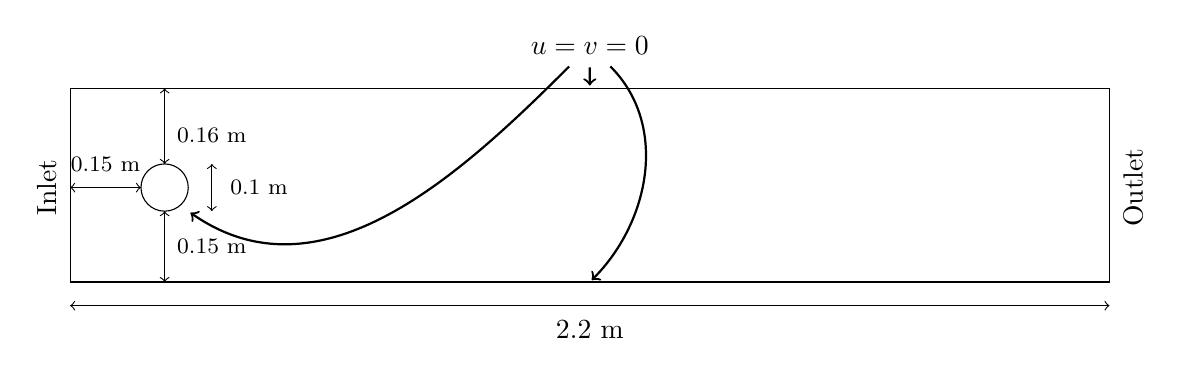
\begin{tikzpicture}[scale=6]
            \draw (0,0) -- (2.2,0) -- (2.2,0.41) -- (0,0.41) -- cycle;
            \draw (0.2,0.2) circle (0.05);
            \draw[<->] (0,-0.05) -- (2.2,-0.05);
            \draw (1.1,-0.1) node {2.2 m};
            \draw[<->] (0,0.2) -- (0.15,0.2);
            \draw (0.075,0.25) node {\footnotesize 0.15 m};
            \draw[<->] (0.2,0) -- (0.2,0.15);
            \draw (0.3,0.075) node {\footnotesize 0.15 m};
            \draw[<->] (0.2,0.25) -- (0.2,0.41);
            \draw (0.3,0.31) node {\footnotesize 0.16 m};
            \draw[<->] (0.3,0.15) -- (0.3,0.25);
            \draw (0.4,0.2) node {\footnotesize 0.1 m};
            \node[rotate=90] (outflow) at (2.25, 0.2) {Outlet};
            \node[rotate=90] (inflow) at (-0.05, 0.2) {Inlet};
            \node (NoFlow) at (1.1,0.5) {$u=v=0$};
            \draw[next] (NoFlow) to (1.1,0.41);
            \draw[next] (NoFlow) to [out=-45,in=45] (1.1,0);
            \draw[next] (NoFlow) to [out=-135,in=-35] (0.25,0.15);
        \end{tikzpicture}
        \caption{Problem Geometry for NSE flow around a cylinder, $\Omega$}
        \label{fig:2DCylinder}
    \end{figure}

    Finally, we choose a simple goal functional, namely the average velocity in
    the $x$-direction, i.e.
    \begin{equation}
        \int_{I}\!\int_{\Omega} u\, d\mathbf{x}\,dt.
        \label{eq:NSEGoal}
    \end{equation}

    For much of this example the code is quite similar to the previous example,
    \autoref{lst:Heat}.  Some differences come from the more complex geometry,
    time dependent boundary conditions, and stabilization. One additional
    complexity is the non-linearity inherent to the Navier-Stokes equations
    which does not exist in the Heat equation. AFES assumes all problems are
    non-linear, and therefore no changes must be made to take into account a
    non-linear problem.  It should, however, be mentioned that this assumption
    by AFES does tend to slow the calculations down for linear problem. As for
    the other complexity added by flow around a cylinder, AFES handles the
    additionally complexity in a straight forward manner that is similar to what
    one would expect in the standard Python interface of FEniCS/DOLFIN.

    The first step we take is setting up problem specific parameters, including
    definition of geometric extent, maximum velocity, etc.
    \lstinputlisting[firstline=6,lastline=15,
        caption={Problem specific parameter definitions for Navier-Stokes
        equation}
    ]{NSE.py}
    Then in the same way we did in the previous example we setup the initial
    conditions and send them to \texttt{Problem}
    \lstinputlisting[firstline=22,lastline=30, label={lst:ICExpNSE},
        caption={Expression for the initial conditions for Navier-Stokes
        equations}
    ]{NSE.py}
    \lstinputlisting[firstline=70,lastline=72, label={lst:ICNSE},
        caption={Initial conditions for Navier-Stokes equations}
    ]{NSE.py}
    \lstinputlisting[firstline=210,lastline=210,
        caption={Passing the initial conditions for Navier-Stokes to
            \texttt{Problem}}
    ]{NSE.py}

    Next we define the various boundaries, which include the inflow, outflow,
    and no-slip boundaries (the cylinder is considered a no-slip boundary), then
    we define the boundary conditions and send this to \texttt{Problem}
    \lstinputlisting[firstline=33,lastline=67, label={lst:SubDomainsNSE},
        caption={Defining problem specific boundaries for flow around a
            cylinder.}
    ]{NSE.py}
    \lstinputlisting[firstline=80,lastline=94, label={lst:BCsNSE},
        caption={Defining boundary conditions for Navier-Stokes equations}
    ]{NSE.py}
    \lstinputlisting[firstline=187,lastline=198, label={lst:DomainNSE},
        caption={Definition of domain and mesh for flow around a cylinder.}
    ]{NSE.py}
    \lstinputlisting[firstline=210,lastline=210, label={lst:BC2ProblemNSE},
        caption={Passing boundary conditions to \texttt{Problem} for
            Navier-Stokes equations flow around a cylinder.}
    ]{NSE.py}

    With the domain and boundary conditions in place we must allow for the
    boundary conditions to be updated. To do this we add the update function to
    \texttt{Problem}, which is done in much the same way as the other functions
    we have added up until now
    \lstinputlisting[firstline=101,lastline=105, label={lst:UpdateBCs},
        caption={Update boundary conditions.}
    ]{NSE.py}
    \lstinputlisting[firstline=214,lastline=214, label={lst:Update2Problem},
        caption={Passing the update function to \texttt{Problem}.}
    ]{NSE.py}

    Next we define the goal functional, \eqref{eq:NSEGoal}, to be used for goal
    oriented adaptivity.
    \lstinputlisting[firstline=108,lastline=113, label={lst:Functional},
        caption={Goal functional.}
    ]{AdaptiveNSE.py}
    And then we send the goal functional to the AFES API and tell AFES to use
    adaptivity.
    \lstinputlisting[firstline=192,lastline=192, label={lst:AdaptiveBool},
        caption={Setting the the adaptive boolean to true.},
    ]{AdaptiveNSE.py}
    \lstinputlisting[firstline=228,lastline=228, label={lst:Goal2Problem},
        caption={Passing the goal functional to the \texttt{Problem} class}
    ]{AdaptiveNSE.py}
    These are the only necessary additions needed for goal oriented adaptivity
    in the Navier-Stokes equation. Most applications of the goal oriented
    adaptivity will be quite similar and won't need any real changes.

    Now that the problem has been defined we then proceed by defining the
    solver. Again the steps here are quite similar to before, except with the
    addition of the stabilization terms. Here the stabilization is given by the
    function \texttt{strong\_residual}, and so this function, in addition to
    \texttt{function\_space} and \texttt{weak\_residual}, must be sent to the
    \texttt{Solver}. This can be seen in the following lines, including the
    passing of the functions \texttt{function\_space}, \texttt{weak\_residual},
    and \texttt{strong\_residual} to the \texttt{Solver} class.
    \lstinputlisting[firstline=120,lastline=187,
        label={lst:AdaptiveWeakFormNSE},
        caption={Function space, weak residual with the \texttt{ei\_mode} used
            to turn off the stabilization and stabilization for the
            Navier-Stokes equation.}
    ]{AdaptiveNSE.py}
    \lstinputlisting[firstline=220,lastline=221, label={lst:Weak2SolverNSE},
        caption={Passing the function space, weak residual, and
            stabilization to \texttt{Solver}.}
    ]{NSE.py}

    The entire code can be viewed below
    \lstinputlisting[label={lst:NSE},
        caption={Complete code for Navier-Stokes flow around a cylinder using
        goal oriented adaptivity.}
    ]{AdaptiveNSE.py}

%\subsection{Optimization} \label{sse:Optimization}
